\documentclass[10pt]{article}
\usepackage{textcomp, graphicx,amssymb, amstext, amsmath, epstopdf, booktabs, verbatim, geometry, appendix, natbib, lmodern, float, tabularx, color}

\geometry{letterpaper}
\usepackage{etoolbox}


\usepackage[utf8]{inputenc}
\usepackage{listings}

\definecolor{codegreen}{rgb}{0,0.6,0}
\definecolor{codegray}{rgb}{0.5,0.5,0.5}
\definecolor{codepurple}{rgb}{0.58,0,0.82}
\definecolor{backcolour}{rgb}{0.95,0.95,0.92}

\lstdefinestyle{mystyle}{
    backgroundcolor=\color{backcolour},
    commentstyle=\color{codegreen},
    keywordstyle=\color{magenta},
    numberstyle=\tiny\color{codegray},
    stringstyle=\color{codepurple},
    basicstyle=\footnotesize,
    breakatwhitespace=false,
    breaklines=true,
    captionpos=b,
    keepspaces=true,
    numbers=left,
    numbersep=5pt,
    showspaces=false,
    stringstyle=\color{codepurple},
    showstringspaces=false,
    showtabs=false,
    tabsize=2
}

\lstset{style=mystyle}

\usepackage{hyperref}
\usepackage{tikz}
\usetikzlibrary{positioning, arrows.meta, calc, fit}

%-----------------------------------------------------------
\newcommand*{\Title}{AgentDesign: Hermes Profile Architecture}
\newcommand*{\cpiType}{Math \& Librarian Profiles --- Design Documentation}
\newcommand*{\Date}{September 2026}
\newcommand*{\Author}{Mehdi Ghasemi}
\newcommand*{\Company}{Research Workspace}
\newcommand*{\Us}{M. Ghasemi}

\newbool{Toptal}
\setbool{Toptal}{false}
\newbool{Guidelines}
\setbool{Guidelines}{false}
\newbool{Proposal}
\setbool{Proposal}{true}

\definecolor{DarkBlue}{rgb}{0,0.2,0.6}
\definecolor{PinkPurple}{rgb}{0.8,0.3,0.3}
\ifbool{Toptal}{
	\hypersetup{
		pdftitle={Project Proposal},
		colorlinks=true,
		linkcolor=toptalGreen,
		filecolor=toptalGreen,
		urlcolor=toptalGreen,
		pdfauthor={Mehdi Ghasemi}
	}
}{
	\hypersetup{
		pdftitle={AgentDesign: Hermes Profile Architecture},
		colorlinks=true,
		linkcolor=DarkBlue,
		filecolor=PinkPurple,
		urlcolor=PinkPurple,
		pdfauthor={Mehdi Ghasemi}
	}
}

\title{\Title}
\author{\Author}
\date{\Date}
%-----------------------------------------------------------
\usepackage{gensymb}
\usepackage{pifont} % \ding for enabled/disabled marks (\mkE, \mkD)
\usepackage{cpistuff/cpi} % This is what makes your document look like a cpi document.

% small helpers for this document — MUST come after cpistuff/cpi (it redefines \mono)
\newcommand{\mono}[1]{{\ttfamily\small #1}}
\definecolor{mathgreen}{RGB}{26,93,58}
\definecolor{libbrown}{RGB}{93,58,30}
\newcommand{\mkE}{\textcolor{mathgreen}{\ding{51}}}       % enabled
\newcommand{\mkD}{\textcolor{PinkPurple}{\ding{55}}}      % disabled
\newcommand{\mkA}{$-$}                                    % absent

\begin{document}

\begin{titlepage}
\maketitle
\end{titlepage}

\linespread{1.2}

\begin{executive}

This document records the complete design of the two Hermes agent profiles that power my
mathematical research workflow --- \textbf{\mono{math}} and \textbf{\mono{librarian}} --- and
specifies an abstraction layer under which either profile can be re-pointed at any future math
project without modification. All facts are extracted from the live configuration on
\texttt{/home/mehdi/.hermes/profiles/} (config version 49, September 2026); every claim in
Sections~\ref{sec:profiles}--\ref{sec:defects} is verifiable against the files listed in
Section~\ref{sec:sources}.

The architecture resolves into five layers: a shared \emph{Hermes core}, an isolated
\emph{profile system}, a \emph{skill catalog} (57--59 skills, capability-gated per profile),
an \emph{MCP bridge} (13 registered servers, one generic CLI-adapter pattern covering 8 of them),
and an \emph{external service plane} on the local network. The math profile is a full-stack
researcher with a 5.9\,GB sandboxed toolchain environment; the librarian profile is a
capability-degraded derivative that shares every registration but disables all computational
skills and adds two ingestion skills of its own.

Two structural findings drive the abstraction design: (i)~the librarian profile's MCP servers
import scripts from the math profile's directory tree, so it cannot exist without the math
profile; and (ii)~both profiles contain a stale reference to \mono{IreneRewrite}, deleted when
that worktree was merged into \mono{Irene} on 2026-09-18. Section~\ref{sec:abstraction}
proposes a capability/manifest model --- persona templates, path interpolation, a shared adapter,
a service registry, and per-project binding files --- that removes every identified coupling in
five concrete steps.

\end{executive}

\tableofcontents
\newpage

%=====================================================================
\section{Objectives and Scope}\label{objectives}

The \mono{AgentDesign} project has three objectives:

\begin{enumerate}
    \item \textbf{Document the as-is architecture.} Record, with file-level evidence, how the
    math and librarian profiles are composed: directory layout, configuration sections, skill
    catalogs, MCP server registrations, external services, scheduled jobs, and state stores.
    This is Sections~\ref{sec:layers}--\ref{sec:workflow}.
    \item \textbf{Identify the coupling points.} Enumerate every place where a profile depends
    on the specific current project layout --- absolute paths, cross-profile imports, hardcoded
    endpoints, and stale references --- so that the design of record distinguishes what is
    load-bearing from what is incidental (Section~\ref{sec:defects}).
    \item \textbf{Specify an abstraction layer.} Define how profiles become reusable personas:
    independent of any particular math project, instantiable for a new project with zero or one
    line of configuration, and testable against a capability contract
    (Section~\ref{sec:abstraction}).
\end{enumerate}

The scope is the two active research profiles. The remaining four registered profiles
(\mono{default}, \mono{coder}, \mono{advisor}, \mono{trader}) are out of scope; their existence
is noted only in Section~\ref{sec:profiles}. This project does not modify any live profile
configuration --- it is a documentation and design artifact.

%=====================================================================
\section{Layered Architecture}\label{sec:layers}

Figure~\ref{fig:layers} gives the visual layout of the infrastructure under which both profiles
operate. Five layers are distinguished; each lower layer is shared, each upper layer is isolated
per profile at \mono{\textasciitilde/.hermes/profiles/<name>/}.

\begin{figure}[H]
\centering
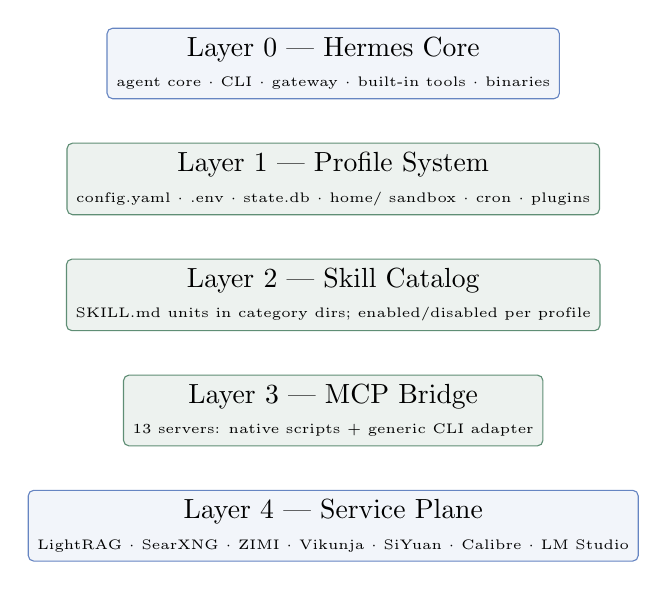
\begin{tikzpicture}[
    boxL/.style={draw=DarkBlue!60, fill=DarkBlue!5, rounded corners=2pt, minimum width=3.1cm, align=center},
    boxP/.style={draw=mathgreen!70, fill=mathgreen!8, rounded corners=2pt, minimum width=3.1cm, align=center},
    layerLbl/.style={font=\small\bfseries, text=DarkBlue},
    every edge/.style={->, >=Stealth, draw=codegray}
  ]
  \node[boxL] (core) {Layer 0 --- Hermes Core\\[-1pt]\tiny agent core $\cdot$ CLI $\cdot$ gateway $\cdot$ built-in tools $\cdot$ binaries};
  \node[boxP, below=.55cm of core] (prof) {Layer 1 --- Profile System\\[-1pt]\tiny config.yaml $\cdot$ .env $\cdot$ state.db $\cdot$ home/ sandbox $\cdot$ cron $\cdot$ plugins};
  \node[boxP, below=.55cm of prof] (skill) {Layer 2 --- Skill Catalog\\[-1pt]\tiny SKILL.md units in category dirs; enabled/disabled per profile};
  \node[boxP, below=.55cm of skill] (mcp) {Layer 3 --- MCP Bridge\\[-1pt]\tiny 13 servers: native scripts + generic CLI adapter};
  \node[boxL, below=.55cm of mcp] (svc) {Layer 4 --- Service Plane\\[-1pt]\tiny LightRAG $\cdot$ SearXNG $\cdot$ ZIMI $\cdot$ Vikunja $\cdot$ SiYuan $\cdot$ Calibre $\cdot$ LM Studio};
\end{tikzpicture}
\caption{Five-layer profile architecture. Layers 2--3 are the capability surface of a profile;
layers 0 and 4 are shared infrastructure. Arrows indicate the direction in which each layer is
configured by, or depends on, the layer above it.}\label{fig:layers}
\end{figure}

\subsection*{Layer 0 --- Hermes Core}
The core lives at \mono{\textasciitilde/.hermes/hermes-agent/}: agent runtime, CLI (profile
switching, tool registry), platform gateway (Telegram/WhatsApp/webhook adapters), built-in tools
(terminal, browser, vision, file I/O, web search, kanban, memory) and the MCP discovery layer
(\mono{tools/mcp\_tool\_*.py}). Shared binaries (\mono{tirith} security scanner, \mono{uv}, Python
3.14, Node 26, ripgrep, Chromium) live in \mono{\textasciitilde/.hermes/tools/}; all MCP stdio
servers run from a single shared virtualenv at \mono{\textasciitilde/.hermes/mcp-servers/.venv/}.

\subsection*{Layer 1 --- Profile System}
Each profile is an isolated directory with its own configuration, credentials, state and sandbox.
The two profiles under study:

\begin{itemize}
    \item \textbf{\mono{math}} (8.4\,GB; 493 sessions): full-stack mathematical researcher.
    Working directory \mono{/home/mehdi/Code/Python/}. Carries a 5.9\,GB sandboxed home
    environment with the complete local toolchain (Section~\ref{sec:profiles}). Active Telegram
    gateway; five cron jobs registered (two enabled). Kanban orchestrator and default assignee is \mono{math}.
    \item \textbf{\mono{librarian}} (174\,MB; 8 sessions): literature manager --- ``manage and
    maintain books and articles.'' Working directory \mono{/home/mehdi/Code/}. Empty \mono{home/}
    stub, no cron jobs, no gateway platforms. Shares the same kanban assignment (\mono{math}), which
    is itself a coupling noted in Section~\ref{sec:defects}. It is also the only profile with an active
    metrics sender: its \mono{telemetry.shared\_metrics} block has both \mono{enabled} and \mono{send}
    set to true; math's config carries no telemetry block at all.
\end{itemize}

Both profiles run the same local model: \mono{qwen3.8-27b} via LM Studio at
\mono{http://localhost:1234/v1}, with an \mono{on\_session\_start} hook
(\mono{\textasciitilde/.hermes/agent-hooks/ensure-lmstudio.sh}) that guarantees the model server
is up before each session. Long-term memory in both profiles is backed by Honcho
(\mono{memory.provider: honcho}, service at port 8008).

\subsection*{Layer 2 --- Skill Catalog}
Skills are Markdown-defined capability units (\mono{SKILL.md} with YAML frontmatter), organized
in category directories, optionally carrying scripts and credential files. Each profile holds 57
skill units across nine named categories plus a handful of top-level skills (union: 59); the full
per-profile inventory is in \mono{references/skill\_inventory.md}; Section~\ref{sec:skills} summarizes
the design-relevant parts.

\subsection*{Layer 3 --- MCP Bridge}
Skills reach services either directly (terminal/shell) or through Model Context Protocol servers
registered under \mono{mcp\_servers:} in each profile's config; every registered tool is exposed
to the model as \mono{mcp\_<server>_<tool>}. Section~\ref{sec:mcp} documents the two server
families and the cross-profile dependency this layer creates.

\subsection*{Layer 4 --- Service Plane}
A fixed set of self-hosted services on the local network (host \mono{192.168.1.70}, DDNS fallback
\mono{mghasemi.ddns.net}), plus two SaaS APIs and one local inference server. Table~\ref{tab:services}
\end{document}
